\sectionLabel{Training and Testing}

\subsectionLabel{Training}

\begin{enumerate}
\item Propose all possible features as candidate features.
\item Prune features that have insufficient data or are uninformative discriminators.
\item Sort remaining features in order of decreasing strength.
\item Store the list of features and their associated statistics for use at run time.
\item Serialize and write the trained model and feature vectors to a file that can be distributed.
\end{enumerate}

A training example consists of a sentence, represented as a set of active
features, together with the word Wc in the confusion set that is correct for
that sentence.

Now that we have a list of proper training data, we train a classifier for each
word in our confusion set. Training proceeds in an on-line manner, each example
is treated as a positive example for the classifiers for \(W_c\), and as a negative
example for the classifiers for the other words in the confusion set.

\lstset{style=sharpc}
\addcontentsline{lot}{table}{\textit{Training} using Debug Corpus example}
\begin{lstlisting}
private class RoughSample
{
    public HashSet<string> Features { get; set; }
    public string Word { get; set; }
}

var cloudClassifiers = new Dictionary<string, ISupervisedLearning[]>(confusionSet.Count());
foreach (var word in confusionSet)
{
    var classifiers = new ISupervisedLearning[1];
    int i = 0;
    for (double beta = 0.5; beta < 1 && i < classifiers.Length; beta += 0.1, i++)
    { classifiers[i] = new Winnow.Winnow(features.Length, threshold: 1, promotion: 1.5, demotion: beta, initialWeight: 1); }
    cloudClassifiers[word] = classifiers;
}
\end{lstlisting}

\begin{figure}[H]
    \centering
    \caption{Training of the models}
    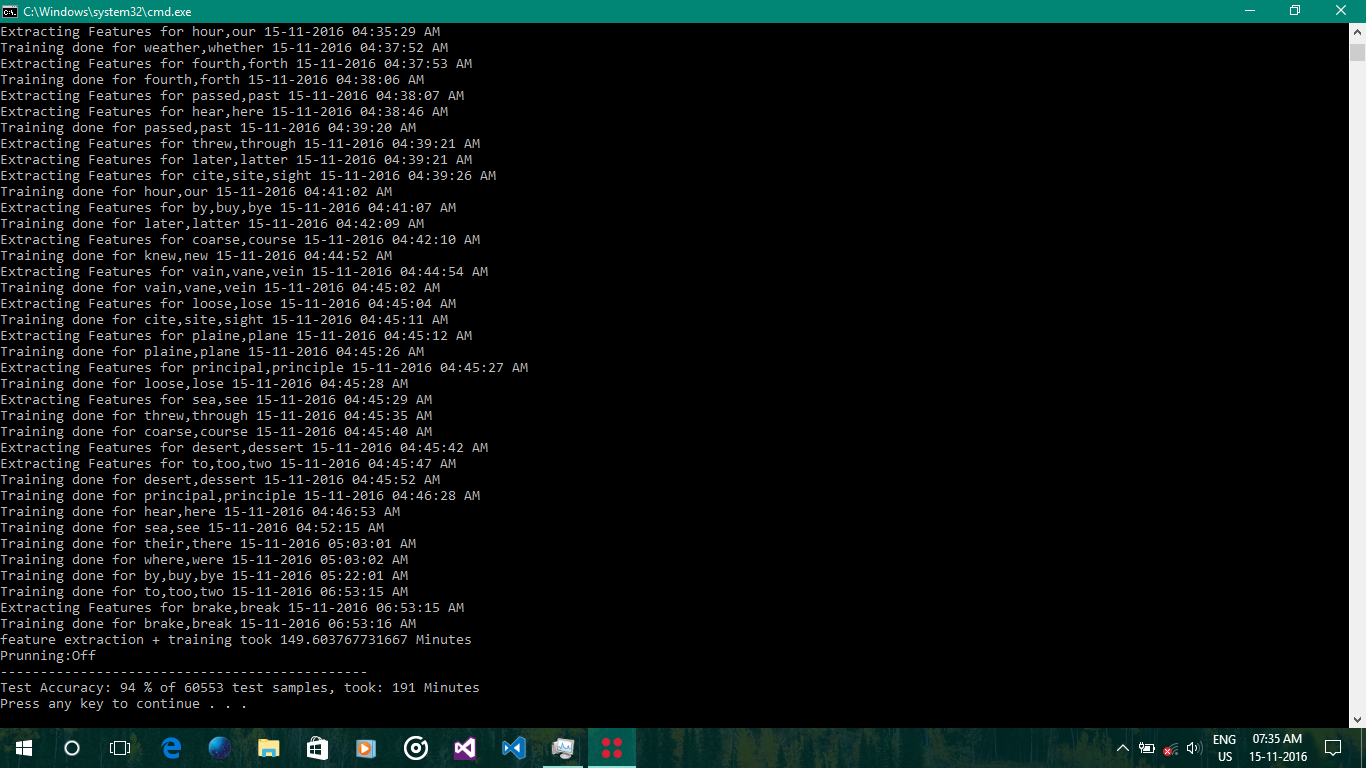
\includegraphics[width=130mm]{img/train.png}
\end{figure}

\subsectionLabel{Testing}

\begin{enumerate}
\item Read the feature vectors and trained model from the serialized file.
\item Read input sentences from a console / file.
\item Pass the sentences to the trained classifier model which makes its corrections, if any.
\item Also pass the sentences to other classifier modules available (Levenshtein distance etc.) and collect their corrections if any.
\item Present the list of corrections to the user as possible corrections.
\end{enumerate}

When a sentence is presented, the system checks the classifiers of each
confusion set, if the sentence contains a word from a confusion set, features
are extracted and run against the corresponding classifier, and returns the
prediction with the highest score.

\begin{figure}[H]
    \centering
    \caption{Correction of a sentence using Context correction}
    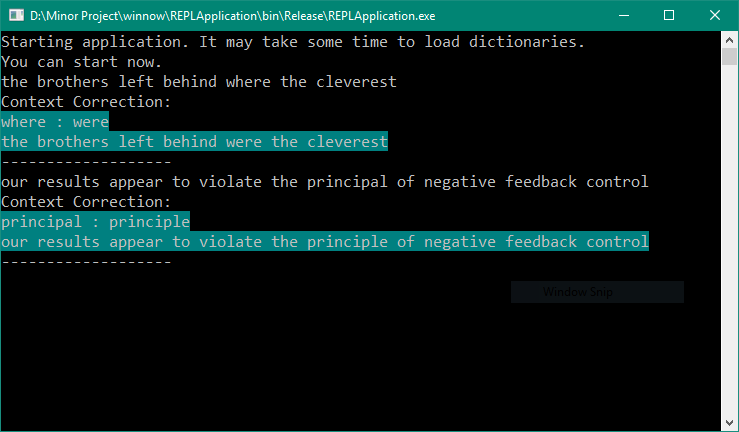
\includegraphics[width=130mm]{img/context.png}
\end{figure}

If the target doesn't accumulate enough features (example may be when the
target word falls at the end of a sentence), the \textit{Edit Distance
corrector} kicks in and tries to find the word from the dictionary or the
confusion sets with the minimum \textit{edit distance}. This helps to ensure
that the predictions can be made with some heuristic even if there is not
enough contextual information available.

\begin{figure}[H]
    \centering
    \caption{Prediction of a sentence using Winnow}
    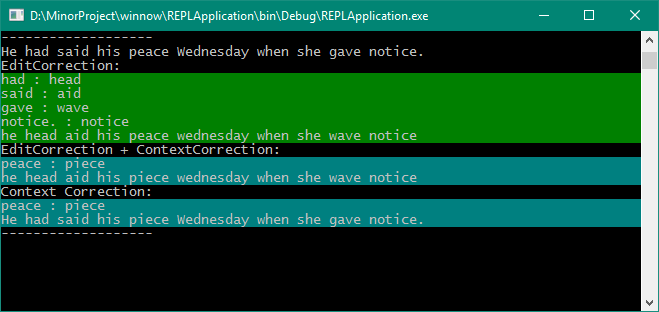
\includegraphics[width=130mm]{img/context+edit1.png}
\end{figure}

